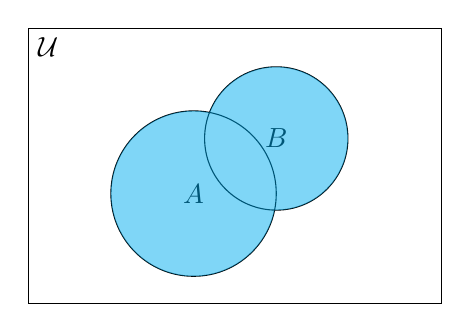
\begin{tikzpicture}[scale=.7]
\draw (0, 0) rectangle (7.5, 5);
\draw (0, 5) node[below right] {$\mathcal{U}$};

\draw (3, 2) circle (1.5cm) node {$A$};
\draw (4.5, 3) circle (1.3cm) node {$B$};
\begin{scope}[fill opacity=0.5]
	\fill[cyan] (3, 2) circle (1.5cm);
	\clip (3, 2) circle (1.5cm) (0, 0) rectangle (7.5, 5);
	\fill[cyan] (4.5, 3) circle (1.3cm);
\end{scope}
\end{tikzpicture}